\documentclass[tikz,border=6pt]{standalone}
\usepackage{pgfplots}
\pgfplotsset{compat=1.18}
\usepgfplotslibrary{colormaps}
\usetikzlibrary{arrows, arrows.meta, calc}
\usetikzlibrary{decorations.markings}

\usepackage{amssymb,amsmath,mathtools}

\usepackage[T1]{fontenc}
\usepackage[utf8]{inputenc}
\usepackage{newpxtext,newpxmath}
\usepackage{sectsty}

\begin{document}
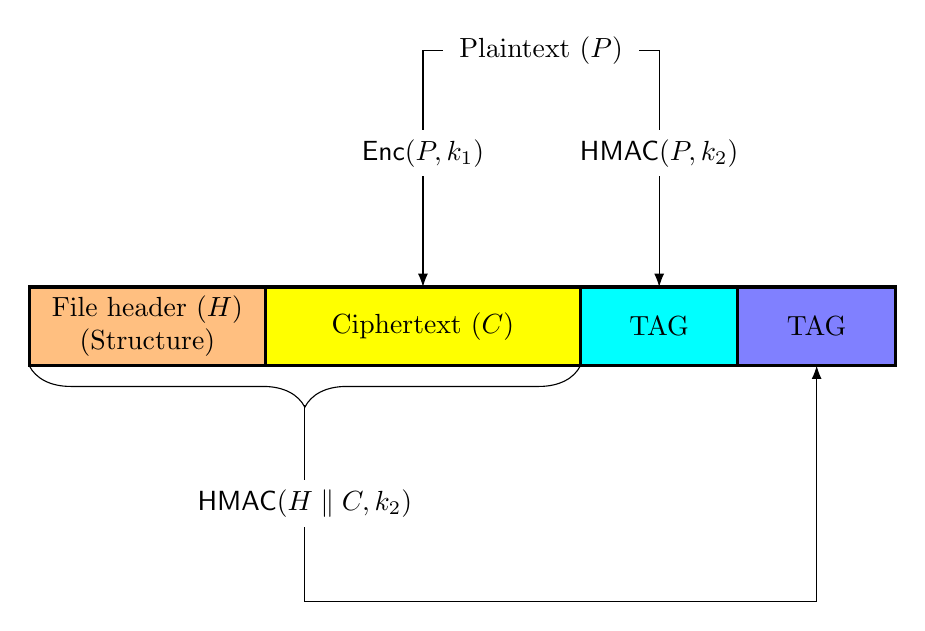
\begin{tikzpicture}[>=Latex, scale=1]
%	\draw[gray!50, dashed, step=1] (-1,-8) grid (12,8);
%	\draw[->] (-1,0) -- (12,0);
%	\draw[->] (0,-8) -- (0,8);
	\draw[line width=.4mm, fill=orange!50] (-1,0) rectangle (2,1) 
	node[midway, black, align=center] {File header $(H)$ \\ (Structure)};
	\draw[line width=.4mm, fill=-blue] (2,0) rectangle (6,1) 
	node[midway, black] {Ciphertext ($C$)};
	\draw[line width=.4mm, fill=-red] (6,0) rectangle (8,1) 
	node[midway, black] {TAG};
	\draw[line width=.4mm, fill=blue!50] (8,0) rectangle (10,1) 
	node[midway, black] {TAG};
	
	\node at (5.5,4) {Plaintext $(P)$};
	\draw[->] (4.25,4) -- ++(-.25,0) -| node[below=1cm, fill=white] {$\mathsf{Enc}(P, k_1)$} ++(0,-3) ;
	\draw[->] (6.75,4) -- ++(.25,0) -| node[below=1cm, fill=white] {$\mathsf{HMAC}(P, k_2)$} ++(0,-3) ;
	
	\draw [decorate,decoration={brace,amplitude=15pt}] (6,0) -- (-1,0);
%	node [below=6pt, midway] {Label for underbrace};
	\draw[->] (2.5,-.5) -- node[fill=white] {$\mathsf{HMAC}(H\parallel C, k_2)$} 
	++(0,-2.5) -- ++(6.5,0) -- ++(0,3) ;
\end{tikzpicture}
\end{document}
